% !TEX TS-program = pdflatex
% !TEX root = ../ArsClassica.tex
\newcommand{\bpic}{$\beta$ Pic b }
\newcommand{\mj}{M$_{j}$}
%************************************************
\chapter{Introduction}
%Meyor queloz
Since the first detection of a planet around a sun-like star \parencite{Mayor1995} the field of exoplanets has evolved rapidly.
Thousands of companions have been identified using the radial velocity and transit detection methods, and a handful have been imaged directly using both ground and space based observatories.
In the last decade, many advances have been made that allow us to begin to characterize the properties of a few of these planets using spectroscopy.
With the launch of the James Webb Space Telescope (JWST) in 2021, and the dawn of the era of extremely large telescopes, we will be able to peer deeper into these planets and further constrain atmospheric or geological properties. 
This will allow us to answer questions about their formation history, climate, and in the long term even the prospects for habitability and life.

JWST will operate in near to mid infrared wavelengths, which will provide a new window into studying the atmospheres of exoplanets and brown dwarfs. 
The Mid Infrared Instrument (MIRI) will provide unprecedented spectral resolution in the mid infrared, allowing for the measurement of composition, pressure and temperature. 
Novel instrumentation does not come without challenges. 
Optical and instrumental effects will constrain the ability to which we can measure spectral features, which will ultimately limit the science that can be accomplished.

In this thesis, we will measure the impact of thin-film fringing in the layers of the detectors in the MIRI Medium-Resolution Spectrometer (MRS) on measurements of atmospheric parameters of brown dwarfs and exoplanets.
This will provide a baseline for determining the level of correction necessary to minimize the impact of fringing, as well as providing a first look into the ability of the MRS to characterize atmospheres through mid-infrared spectroscopic observations, and using modern atmospheric retrieval techniques.

\section{Exoplanets}
The last quarter century of observations has revealed the diversity of exoplanets and extra-solar systems.
Both the architecture and individual planetary characteristics vary greatly when compared to each other, as well as to our own solar system.
From the hot Jupiters initially found by Mayor and Queloz \parencite{Mayor1995} to the thousands of planets discovered by the Kepler mission, the variety in exoplanets has raised questions about their formation and development, as well as their present day structure and climate.
Improvements to observational techniques have allowed us to improve our understanding of these planets.
Secondary eclipse and transmission spectroscopy has opened the door to the study of planets in close orbits to their host stars, while emission spectroscopy of young planet has allowed for constraints on models of planet formation.
Over the next decades new instruments will be developed that improve sensitivity, allowing us to study smaller, colder and fainter planets.
This will address one of the ultimate goals of exoplanet science in studying the atmospheric and surface features of an earth-like planet in the hopes of detecting unambiguous biosignatures.

Of particular interest are observable features that allow us to measure physical properties of exoplanets.
The radial velocity (RV) method provides a measure of the planet mass, while a transit can constrain the radius.
Already these properties tell us something about the overall structure of the planet.
Spectroscopy can provide insight into the composition of the planet's atmosphere, as well as its temperature and pressure.
These properties are linked to its age and location of formation in the circumstellar disk.
The atmosphere, combined with the distance between the planet and its star determine the climate of the planet.

%Exoplanet Science Strategy Text: state of field, goals, timelines, summary of methods, biosignatures, formation, tracers, methods, parameters of interest.
% Kepler, Tess, Cheops, RV
\subsubsection{Direct Imaging}
While the majority of exoplanet detections have been made using the radial velocity or transit techniques, direct imaging opens up the possibility of collecting light from the planet itself.
This provides a window into the planet's atmosphere and surface.
Most direct imaging to date has used near-to-mid infrared wavelengths, where the contrast between the thermal emission from the planet and the star is at a minimum, as in Fig. \ref{fig:solarsystem}.
This has its drawbacks: we are so far only able to image young planets that have retained some of the heat from their formation.
 
\begin{figure}[t]
	\centering
	\includegraphics[width=0.9\linewidth]{familyphoto.png}
	\caption{A family portrait of some of the directly imaged exoplanets.
		In order:
	\parencite{Marois2010}, \parencite{Rameau2013}, \parencite{Stolker2020}, \parencite{Sallum2015}, \parencite{Keppler2018}, \parencite{Currie2012}, \parencite{Macintosh2015}, \parencite{Chauvin2004}, \parencite{Quanz2010}.}
	\label{fig:family}
\end{figure}

Direct imaging can make use of both ground and space based observatories. 
However, the high spatial resolution required drives the need for a large primary mirror, limiting the possibilities of space-based telescopes. 
On the other hand, atmospheric turbulence necessitates the use of an adaptive optics equipped facility to observe from the ground. 
Atmospheric absorption due to telluric lines (absorption lines of Earth's atmosphere) along with the strong background due to thermal emission from the ground and atmosphere also restrict infrared observations to narrow bands.

In addition to the requiring high spatial resolution, it is also challenging to separate the light emitted by the planet from that of the star.
Imaging techniques such as Angular Differential Imaging (ADI) \parencite{Marois2006} and Reference Differential Imaging (RDI) \parencite{Lafreniere2009,Soummer2011} provide methods for reducing the stellar point-spread-function (PSF). %\parencite{Macintosh2006} %ADI
Coronagraphs are optical elements which suppress the stellar PSF through self-destructive interference or physical occultation, depending on the position in the optical path.
The difference in spectra between the planet and the star can also be used to separate the two sources.

\begin{figure}[t]
	\centering
	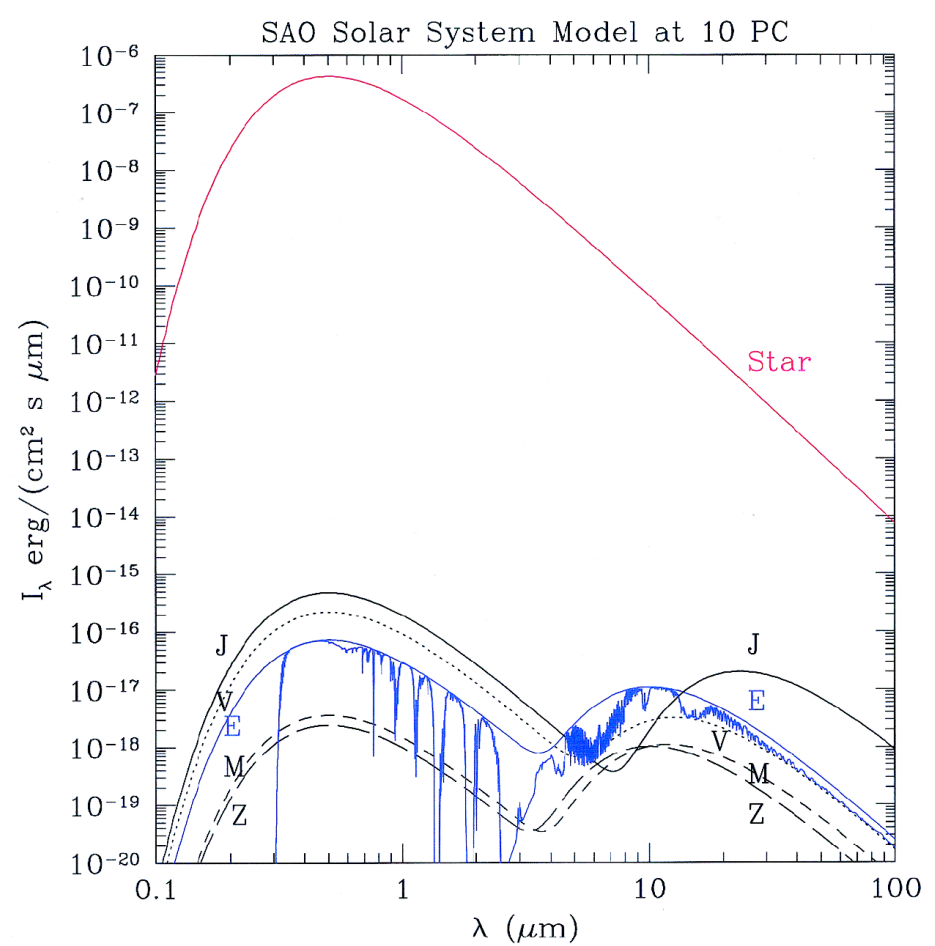
\includegraphics[width=9cm]{solarsystemcontrast.png}
	\caption{SAO solar system model at 10pc, illustrating the vast difference in luminosity between the Sun and the surrounding planets. However, in the mid infrared the contrast is dramatically reduced at the peak of the planet's emission spectra \parencite{DesMarais2002}.}
	\label{fig:solarsystem}
\end{figure}
Presently, 10m class telescopes such as the Very Large Telescope (VLT) in Paranal, Chile or the Gemini Observatory split between Hawaii and Chile provide the best combination of resolution and instrumentation to perform direct imaging of exoplanets.
The NACO instrument at the VLT provided the first image of an exoplanet in 2004 \parencite{Chauvin2004}.
These observatories are among those equipped with an adaptive optics system, coronagraphic instrumentation and near to mid infrared imaging and spectroscopic capabilities to directly image exoplanets, with several exemplar systems becoming standard objects of interest.
While it's terribly interesting to explore the details of each of these objects, we will focus our discussion on objects will be used further in this study, due to their scheduled observation as part of the JWST GTO and Early Release Science (ERS) programs \parencite{Beichman2019}. 
The parameters of these and other directly imaged exoplanets and brown dwarfs are summarized in table \ref{tab:exoplanetparams}. 

In order to understand these objects, we must use a measured spectrum in order to infer physical properties.
Parameters such as the carbon-to-oxygen (C/O) ratio provide insight into formation mechanisms \parencite{Madhusudhan2012}.
A planet that forms near its star will form in a hot region of the circumstellar disk, with a depletion of volatiles due to the high temperature - various species will freeze out at different radii within the disk. 
The measured C/O ratio of a planet will thus depend on its initial formation location and its migration path.
\parencite{Turrini2015} outlines several formation pathways and how the C/O ratio will be affected.
The current climate of exoplanets is also of interest. This requires inferences of atmospheric composition and structure from the spectrum, and will ultimately require time resolved measurements in order to study dynamics and variability. 


 %Not 2019 - summary of JWST science and instruments
 %Exoplanet characterization with JWST MIRI white paper
\subsubsection{VHS-1256 b}
\begin{wrapfigure}{r}{5.5cm}
	\centering
	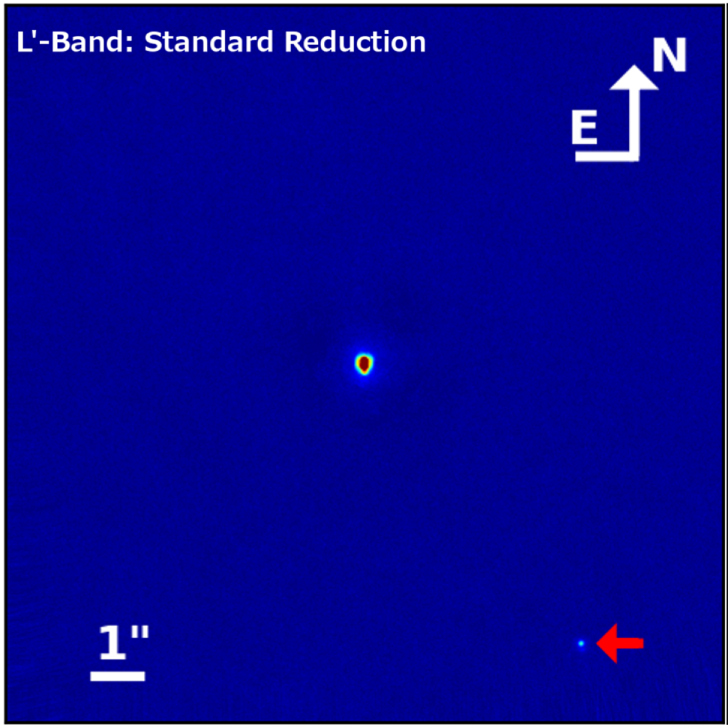
\includegraphics[width=5.2cm]{vhs1256b.jpg}
	\caption{VHS-1256b as observed with Subaru/IRCS in the L'-band \parencite{Rich2016}, reduced using the LOCI algorithm \parencite{Galicher2011}.}
\end{wrapfigure}
Originally discovered in 2015 \parencite{Gauza2015} as part of the VISTA Hemisphere Survey, VHS-1256b is a late-L dwarf in a 102 AU orbit around an M dwarf.
\parencite{Gauza2015} present astrometric, photometric and spectroscopic data on the planet, finding an age of 150-300 Myr from a moving group association, a luminosity log($L_{bol}/L_{\odot}$) of -5.05$\pm0.22$ and infer a mass of 11.2$^{+9.2}_{-1.8}$ M$_{J}$. 
The effective temperature is found to be 880$^{+140}_{-110}$ K from evolutionary models. 
This is substantially colder than field dwarfs of a similar spectral type (typically 1400K), and so it is proposed that a thick Fe and Mg-Si cloud layer acts to reduce the effective temperature.
Similar findings are presented by \parencite{Rich2016} using Subaru/IRCS.

In \parencite{Miles2018}, methane is detected using KECK/NIRSPEC in the L-band. 
The shallow depth of the feature indicates chemical disequilibrium in the photosphere, as the derived abundance departs from an equilibrium abundance by a factor of 10-100.
However, the best fit model retrieves substantially different parameters for temperature (1240 K) when compared to previously published results.

The wide separation (8") and proximity to Earth make VHS-1256b an ideal target for studying atmospheric properties.
It will be observed as part of the JWST ERS Program \parencite{Hinkley2019}, where a medium resolution spectrum (R$\geq$1700) will be measured from 0.6-28 micron. 
This will enable a more precise measurement of the abundance of methane and other species in the atmosphere, and will allow for investigation of the cloud properties in the mid infrared.
\subsubsection{2M1207b}
Using VLT/NACO, \parencite{Chauvin2004} discovered a low mass companion to the brown dwarf 2MASSWJ 1207334-393254 (2M1207) at a separation of 0.8", or 55 AU, shown bottom-center in Fig \ref{fig:family}. 
From their H,K and L'-band photometric observations and NIR spectroscopic measurements, 2M1207b was found to have a spectral type of L5-L9.5, a mass of 5$\pm2$ M$_{J}$ and an effective temperature of 1250$\pm$200 K. Followup VLT/NACO observations from \parencite{Mohanty2007} found a higher effective temperature of 1600$\pm$100 K, and a higher mass of 8$\pm$2 M$_{J}$, pushing it closer to the deuterium burning limit. More recent observations have measured periodic signals due to rotation and variability, but failed to constrain the rotation rate due to pointing variance \parencite{Zhou2019}. 

\parencite{Zhou2019} also present simulated JWST/NIRCAM observations of 2M1207b. Access to medium resolution spectroscopy in the mid infrared will allow the characterization of cloud condensate properties. 
The improvement in photometric precision by an order of magnitude will allow better measurement of the rotation rate and variability, and the increase in sensitivity will place lower limits on the possibility of further companions within the system.
It will be observed as part of the JWST GTO program \parencite{Birkmann2019}.

\begin{landscape}
	\begin{table}[t]
		\centering
		\begin{small}
			\begin{tabular}{lllllllll}
				\toprule
				%Name, Mass, Luminosity, Age, Separation, Sep AU, Pri Mass
				\textbf{Name} & \textbf{d [pc]} & \textbf{Mass [M$_{J}$]} & \textbf{Sep [AU]} & \textbf{Sep ["]} & \textbf{Age [Myr]} & \textbf{log(L$_{bol}$/L$_{\odot}$)} & \textbf{T$_{eff}$ [K]} & \textbf{References}\\
				\midrule
				\multicolumn{9}{c}{\textbf{Widely separated companions}}\\
				\midrule
				VHS 1256b & $12.7\pm1.0$  & $2\pm1$     & $102$ & $8.1$ & $10^{3}-10^{4}$ & $-5.05\pm0.22$ & $880$ & \parencite{Gauza2015}\\
				Fomalhaut b & $7.704\pm0.028$ & $\leq 2$ & $119$ & $13$ & $440\pm40$ & \ldots & $1600\pm100$ &\\
				\midrule
				\multicolumn{9}{c}{\textbf{Close in companions}}\\
				\midrule
				2M1207b   & $152.4\pm1.1$ & $2\pm1$     & $41$ & $0.8$ & $10\pm3$ & $-4.68\pm0.05$ & $1600\pm100$ &\\
				51 Eridani b & $29.4\pm0.3$ & $2\pm1$   & $13$ & $0.45$ & $23\pm3$ & $-5.06\pm0.2$ & $700$ &  \parencite{Macintosh2015}\\
				\bpic     & $19.3\pm0.2$  & $2\pm1$     & $9$ & $0.4$ & $23\pm3$ & $-3.78\pm0.03$ & $1600\pm100$ & \parencite{Quanz2010}\\
				GJ 504b   & $17.56\pm0.08$  & $3-30$    & $44$ & $2.5$ & $100-6500$ & $-6.13\pm0.03$ & $544$ & \parencite{Skemer2016}\\
				HD 95086b & $90.4\pm3.3$  & $5\pm2$     & $56$ & $0.6$ & $17\pm4$ & $-4.96\pm0.10$ & $1050$  &\parencite{DeRosa2016}\\	
				HR8799b   & $39.4\pm1.0$  & $5\pm1$     & $68$ & $1.7$ & $40\pm5$ & $-5.1\pm0.1$ & $870^{+30}_{-70}$ & \parencite{Marois2008,Skemer2012}\\
				HR8799c   & $39.4\pm1.0$  & $7\pm2$     & $38$ & $0.95$ & $40\pm5$ & $-4.7\pm0.1$ & $1090^{+10}_{-90}$ &\parencite{Marois2008,Skemer2012}\\
				HR8799d   & $39.4\pm1.0$  & $7\pm2$     & $24$ & $0.62$ & $40\pm5$ & $-4.7\pm0.2$ & $1090^{+10}_{-90}$ &\parencite{Marois2008,Skemer2012}\\
				HR8799e   & $39.4\pm1.0$  & $7\pm2$     & $14$ & $0.38$ & $40\pm5$ & $-4.7\pm0.2$ & $1000$ &\parencite{Marois2008,Skemer2012}\\	
				LkCa 15b  & $145\pm15$    & $6\pm4$     & $20$ & $0.08$ & $2\pm1$ & \ldots & \ldots &\\
				PDS 70b   & $113.43\pm0.52$ & $7\pm2$   & $23$ & $0.19$ & $5\pm1$ & \ldots & $900$ &\parencite{Haffert2019}\\
				PDS 70c   & $113.43\pm0.52$ & $4.4\pm1$ & $30$ & $0.24$ & $5\pm1$ & \ldots &  $10^{4}$ & \parencite{Haffert2019}\\
				\midrule
				\multicolumn{9}{c}{\textbf{Nearby Brown Dwarfs}}\\
				\midrule
				WISE 0855   & $2.2\pm0.2$ & $3-10$ & \ldots & \ldots & $10^{3}-10^{4}$ & $-10.5$ &  $225-260$ & \parencite{Luhman2014,Tinney2014}\\
				Luhman 16B   & $1.998\pm0.0004$ & $28.6\pm0.3$ & \ldots & \ldots & $600-800$ & $-4.68$&  $1201$ & \parencite{Sahlmann2015};\\
																								&&&&&&&&\parencite{Garcia2017}\\
				\bottomrule
			\end{tabular}
		\end{small}
		\caption{Summary of directly imaged planet and brown dwarf parameters based on \parencite{Bowler2016} and references therein. Luminosity for WISE 0855 is calculated in H band.}
		\label{tab:exoplanetparams}
	\end{table}
\end{landscape}
\section{Brown Dwarfs}
Brown dwarfs are the low mass result of a failed star formation process.
On the low end of the mass scale, an object is considered a brown dwarf at >13M$_{J}$, which is the deuterium burning limit. 
Recent observations of low mass (~1 M$_{J}$), free floating observations have led to challenges of this definition defining the boundaries between planets and brown dwarfs.
By 75M$_{J}$, the object is heavy enough to sustain hydrogen fusion and the object is considered a star.
However, there have recently been observations even lower mass brown dwarfs, down to several Jupiter masses, raising questions of formation processes \parencite{Luhman2014}.
It is generally thought that brown dwarfs form during the gravitational collapse of a molecular cloud, while exoplanets form through a core accretion process in a circumstellar disk.
Observations of high mass companions and low mass field objects then challenge these standard models.

While brown dwarfs are objects of scientific interest in their own right, we are particularly interested in their use as analogs for exoplanets due to their similar temperatures and pressures.
Without the issue of contrast between an exoplanet and its host star, brown dwarfs are ideal targets for medium and high resolution spectroscopic characterization.
As shown in table \ref{tab:exoplanetparams}, they are also some of the closest known objects to the solar system, with several having been observed at around 2pc.

\subsection{Observational Properties}
Brown dwarfs are characterized by their spectral type, either by comparison to spectral templates, using indices derived from spectral parameters or through broadband photometric comparison \parencite{Helling2014}.
Directly imaged exoplanets can also be classified using brown dwarf spectral types.
Unlike stars which maintain their temperature and luminosity through fusion, brown dwarfs cool and change their spectral type with age, leading to a degeneracy between mass and age \parencite{Burrows2001}.
This spectral series is shown in Fig. \ref{fig:bdspec}.

As a brown dwarf cools and contracts over time, its surface gravity will increase, leading to the use of log(g) as a tracer of age \parencite{Manjavacas2014}.
Young, low surface gravity objects are particularly comparable to directly imaged exoplanets.
In these young objects, clouds are a nearly universal feature \parencite{Cooper2003,Helling2014}, with thicker cloud decks appearing in low gravity objects \parencite{Helling2014}.

\begin{figure}[t]
	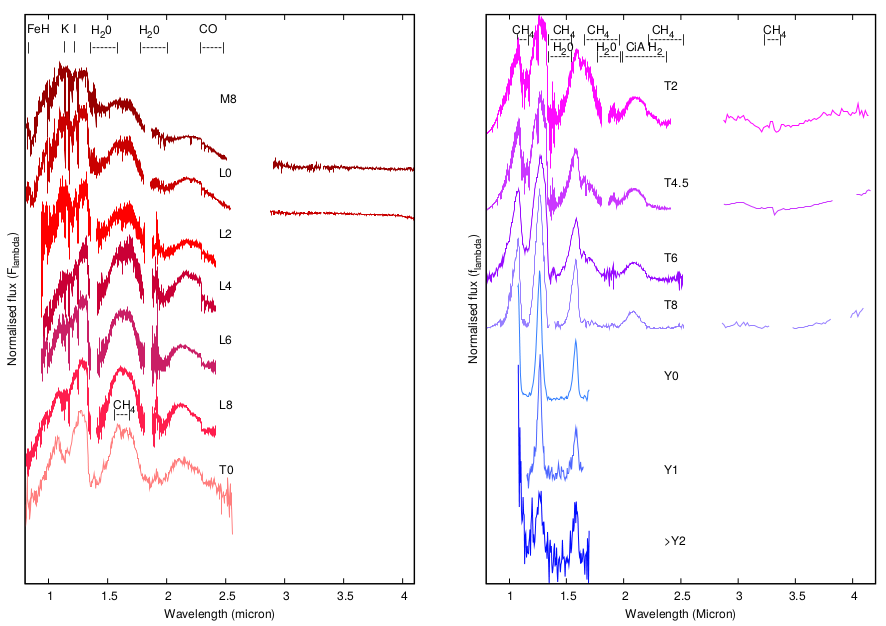
\includegraphics[width=\linewidth]{bdspectral.png}
	\caption[Brown Dwarf Spectra]{Near Infrared spectral series of brown dwarfs from early-M to early-Y as shown in \parencite{Helling2014}.}
	\label{fig:bdspec}
\end{figure}

\subsubsection{L-Type}
L-dwarfs are the hottest brown dwarfs, with typical effective temperatures between 1300 K and 2100 K \parencite{Burrows2001}.
L-type spectra are notable for the disappearance of VO and TiO NIR absorption lines and the onset of molecular absorption features such as H$_{2}$O and CO, with CH$_{4}$ appearing in late L types \parencite{Manjavacas2014}.
Further key features of L-dwarfs is the formation of iron and silicate condensate, as well as the growth of neutral alkali lines \parencite{Burrows2001}.
\subsubsection{T-Type}
As a brown dwarf ages it moves towards a T-type spectrum. 
The L/T transition occurs  with the appearance of both CH$_{4}$ and CO absorption, and is characterized by increasingly blue J-H colour as the temperature decreases.
There are several proposed mechanisms for this transition, with cloud fragmentation due to particle microphysics \parencite{Burningham2017} and convection processes being two examples \parencite{Tremblin2015}.
Both T- and L-dwarfs are highly variable due to complex atmospheric dynamics ranging from clouds to banding structures to hot spots and more \parencite{Biller2017}.
\parencite{Vos2019} presents how monitoring with JWST/MIRI will be able to constrain the mechanism behind this transition.
\subsubsection{Y-Type}
Y-type dwarfs are ultra-cool objects first discovered in \parencite{Cushing2011}. 
With such cold temperatures, they contain deeper water and methane absorption features than present in T-dwarfs, and likely have ammonia present as well.
Atmospheric models suggest typical temperatures between 300-500 K, which places them as the coldest detected and spectroscopically measured brown dwarfs to date \parencite{Cushing2011}.
Due to the very low temperatures of Y-dwarfs, mid-infrared observations are ideal for detection and characterization.
Most spectral features of interest (CH$_{4}$,NH$_{3}$,etc) will be present at longer wavelengths, while the mid infrared will also present opportunities for measurements of cloud properties and composition.

\clearpage
\subsubsection{WISE 0855-0714}
\begin{wrapfigure}{r}{5.5cm}
	\centering
	\vspace{-1em}
	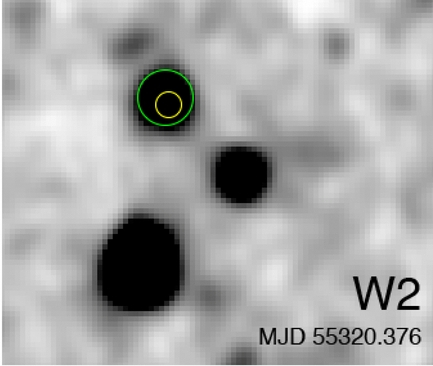
\includegraphics[width=5.2cm]{wise0855im.jpg}
	\caption{W2, epoch 1 image of WISE0855 on top of a known background clump. The green circle represents the location of WISE0855, the yellow is the position of the background source \parencite{Wright2014}. }
	\label{fig:wise0855im}
	%\vspace{-4em}
\end{wrapfigure}
WISE-0855 is the coldest known brown dwarf at 250 K, with an inferred mass of 5 M$_{J}$ \parencite{Luhman2014}, and a Y2-4 spectral type \parencite{Leggett2015}.
Although faint, with a J-band magnitude of 25, its proximity to the sun makes allows for its spectral characterization.
Present measurements indicate the presence of ammonia \parencite{Leggett2015} and water clouds \parencite{Morley2014,Faherty2018} in its atmosphere.

WISE 0855, along with other Y-dwarfs will be the subject of JWST investigation \parencite{Oliveira2015,Oliveira2019}.
Its low mass and cold temperature make it the closest analog to solar system objects, especially to Jupiter. 
Further observations will allow for tighter constraints on atmospheric composition and cloud properties, as well as insight into whether such objects are the result of a star-like formation process or are an ejected, free floating planet \parencite{Beichman2014}.
\section{Motivation}
\subsection{Current Status of Atmospheric Characterization}
Both exoplanets and brown dwarfs raise interesting questions with regards to atmospheric properties, but there are substantial challenges both in gathering the data necessary to answer them and modeling the physics underlying the observable parameters. 
The best methods currently in use involve taking spectroscopic data and inferring atmospheric properties from the spectral features.
The light we measure may be thermal emission from the planet, where it is absorbed and scattered as it passes through the planet's atmosphere, or it may be light from the planet's host star which passes through the upper layers of the atmosphere.
These provide complementary information about the composition and structure of the atmosphere, probing different altitudes and pressures.
While a more complete overview of exoplanet atmospheres is covered in the literature, e.g. \parencite{Bozza,Madhusudhan2014,Seager2010}, we will briefly summarize the current methods used and what has been learned so far.
%Transmission spectroscopy, facilities, atmosphere, climate, condensates
 % Exoplanet atmosphere measurements, hr8799 photometry/spec, prospects for jw
 %Exoplanet atmospheres textbook: observation, models, spectroscopy, solar system atmospheres
 %Atmospheric char with MIRI (coron,LRS, not MRS I think)
%\parencite{Madhusudhan2016} %Chemistry, Formation, Habitabiltiy
\subsubsection{Transmission Spectroscopy}
Many exoplanets have been discovered using the transit technique in which the planet passes in front of its host star, blocking a small fraction of its light.
Through time series observations, particularly with satellites such as Hubble, Kepler, and TESS, we can observe this dip in stellar brightness, and infer properties of the planet.
A key feature of this observation is that in the case the planet has an atmosphere, the brightness dip is wavelength dependent.
Depending on the wavelength, different species within the atmosphere will absorb the light to a greater or lesser extent.
Thus if a species is abundant within the atmosphere, it will create deep absorption features, which will make the apparent radius of the planet larger, increasing the transit depth.
Measuring this radius variation is the procedure of transmission spectroscopy, and is used to probe the composition and structure of the upper atmospheres of transiting planets.
In addition to transmission spectroscopy, secondary eclipse spectroscopy is another transit measurement that uses the reflected light and thermal emission of the planet, and measures the dip in total luminosity as the planet passes behind its host star.
This provides a more direct measurement of the planet's reflection or emission spectrum.
\parencite{Kreidberg2018} presents a concise overview of transmission and eclipse spectroscopy.

Transmission spectroscopy attempts to answer questions about atmospheric composition, formation history and present climate.
To date, water features and carbon-bearing molecules have been detected, though molecules commonly present in the solar system such as methane and ammonia have not been detected, largely due to lack of long wavelength coverage and the high temperatures of most transiting planets \parencite{Lee2012,Kreidberg2018}.
The C/O ratio has been measured in some hot Jupiters, including WAST-12b, which provides a trace for formation history and current composition \parencite{Madhusudhan2011}. 
For WASP-12b, the high C/O ratio (>1) and the lack of an observed thermal inversion in the highly irradiated atmosphere both stand in contrast to theoretical predictions, and demonstrate the necessity for improvements in atmospheric and formation modeling \parencite{Madhusudhan2011}.
In other atmospheres, nitrogen chemistry has been observed, and condensates (clouds and hazes) are nearly universal \parencite{MacDonald2017}.
Water has been detected on hot Jupiters \parencite{Kreidberg2014}, as well as on smaller planets within the `habitable zone' \parencite{Benneke2019,Tsiaras2019}.

Future observations will increase the spectral resolution of transit observations, and will also extend the wavelength coverage. 
By probing the mid infrared, it may be possible to determine the composition of the clouds observed, and place tighter constraints of the abundances of species present within atmospheres \parencite{Kreidberg2018}.

\subsubsection{Emission Spectroscopy}
In contrast to transit observations, emission spectroscopy is a direct measurement of the light emitted by the planet, usually in the infrared, where the planet's luminosity peaks due to Wein's law.
Due to the low levels of flux emitted from most planets, most emission spectroscopy to date has been low to medium resolution, in order to collect enough light for measurement. 
However, this has already allowed us to begin to answer similar questions as posed for transmission spectroscopy.
What are these atmospheres made of? How did these planets form?
In many ways though, emission and transmission spectroscopy provide complementary information, and multiple ways of approaching these problems. 
Due to the different wavelength regimes, they are able to identify different species and probe different atmospheric depths. 

Only recently has high quality exoplanet emission spectroscopy become possible, and a comprehensive overview is provided in \parencite{Biller2018}.
Measurements of H$\alpha$ emission in LkCa 15b have allowed for inferences of the mass accretion rate of a forming planet \parencite{Sallum2015}, while observations of the PDS 70 system indicate the presence of a circumplanetary disk around PDS 70b \parencite{Keppler2018,Christiaens2019}.
With integrated field spectroscopy, \parencite{Hoeijmakers2018} show how spectroscopy can identify the presence of molecular species in a spectrum and how this can be used to discover companions within the contrast-limited regime.
Using the VLTI/GRAVITY instrument, which combines light from all four Unit Telescopes (UTs) of the VLT into a single interferometer, medium resolution (R=500) spectra have been taken of HR 8799e \parencite{Lacour2019} and \bpic \parencite{GRAVITYCollaboration2019}, the latter of which is shown in Fig. \ref{fig:gravitybpic}. 
These spectra represent some of the best data available to date for exoplanets, and additional observations of well-known directly imaged planets are planned in the near future.
With such spectra, atmospheric retrievals are used to infer properties of interest using Bayesian inference, fitting parameterized 1D atmospheric models to the spectrum in order to find the most likely value of those parameters \parencite{Madhusudhan2009}. 
While not yet accomplished for an exoplanet, it may be possible in the near future to longitudinally map cloud features of exoplanets, as has already been accomplished for brown dwarfs using the CRIRES instrument \parencite{Crossfield2014}.
\begin{figure}[t]
	\includegraphics[width=\linewidth]{gravitybpic}
	\caption{Flux calibrated K-Band emission spectrum of \bpic as measured using the VLTI/GRAVITY at R=500 \parencite{GRAVITYCollaboration2019}, along with the GPi K-Band spectrum from \parencite{Chilcote2017}.}
	\label{fig:gravitybpic}
\end{figure}\\

As most older planets will emit primarily in the thermal infrared, JWST/MIRI will provide unprecedented capabilities at imaging and characterizing these systems.
\parencite{Danielski2018} shows that the MIRI Low Resolution Spectrometer will allow for the detection of ammonia in the coldest targets, as well as characterize the abundances of other molecules such as CH$_{4}$, H$_{2}$O, CO$_{2}$ and PH$_{3}$.
Many direct imaging observations of exoplanets have been proposed as part of the JWST GTO and ERS programs. In a white paper, \parencite{Beichman2019} discuss how JWST will provide new insight into exoplanet atmospheres using direct emission imaging and spectroscopy, while \parencite{Line2019} examines the possibility of characterizing terrestrial planets using thermal emission spectroscopy. 

\subsection{JWST Studies}
With the launch of JWST imminent, many proposals have been made to cover a wide range of science cases, as well as performing instrumental testing, calibration and validation.
Exoplanet science is well represented within these first observations, and several of the proposals will be presented here.
\subsubsection{Early Release Science}
The Early Release Science program is an initiative designed to help scientists develop an understanding of the instruments available on JWST, as well as the tools needed to process the data. 
Thus the ERS provides an extensive catalog of public data immediately upon observation, and will take place within the first 5 months of JWST science operations.
Both a transiting program \parencite{Bean2018} and a direct imaging program \parencite{Hinkley2019} have been approved.
The direct imaging proposal has 52 hours observing time in order to take data using the full range of JWST instrumentation and observing modes.
The goal is to image a representative sample of known directly imaged planets, in order to develop the tools and techniques necessary to push the limits of the instrumentation.
For a subset of the imaged planets, including VHS-1256b, spectroscopic data covering the full wavelength range of JWST will be taken using a combination of the available instruments.

\subsubsection{GTO Programs}
In addition to the ERS program, the Guaranteed Time Observations (GTO) program is designed to provide scientists who helped in the development of JWST hardware and software with a set amount of observing time. 
Many GTO programs focused on exoplanet science have been approved, including spectroscopic studies of 2M1207b and other commonly studied systems \parencite{Birkmann2019}.
Brown dwarf science is also well represented within the GTO program, with WISE-0855 receiving full spectroscopic coverage from 0.6-28 $\mu$m \parencite{Oliveira2019}.
Details of the observations for VHS-1256b, 2M1207b and WISE-0855 are discussed in \ref{sec:obs}.

\subsection{Biosignatures and Future Missions}
While JWST will provide higher spectral and spatial resolution in the infrared than any previous observatory, many questions will remain open for future missions.
One of the ultimate unanswered questions in science is "Are we alone?".
The detection of biosignatures in the near future with next generation 40 m class telescopes \parencite{Lopez-Morales2019} or proposed space missions such as LIFE \parencite{Quanz2019} and LUVOIR \parencite{Luvoir2019} may provide our best chance at answering such questions.
Instruments such as METIS on the ELT will offer high resolution (R=100000) integral field spectroscopy of nearby terrestrial planets, while both proposed space missions will have the spatial and spectral resolution necessary to characterize a nearby earth like planet.
With such a goal in mind, it is necessary to develop the technical capabilities in both theory and observation order to achieve such ambitious goals in the not-so-distant future.

\section{Thesis Overview}
With sufficient background and motivation, we will now outline the remainder of this thesis.

Chapter 2 will provide a more extensive background of the James Webb Space Telescope, and in particular the MIRI Medium Resolution Spectrometer (MRS).
We will outline the principle optical components dedicated to integral field spectroscopy, as well as the detector characteristics of MIRI.
This will provide the necessary background to understand the instrumental and optical effects discussed in Chapter 3.

The third chapter examines the fringing effect in the MIRI MRS instrument.
We discuss the optical effects that result in fringing patterns, as well as outlining current and future strategies for fringe correction.
We describe the creation and processing of our mock observations using the MIRI instrumental simulator and the JWST data reduction pipeline.
With the degraded spectra from the simulated data, we measure the impact of fringing on spectral extraction using cross correlation techniques, and and how this impacts molecular mapping studies.
This in turn motivates Chapter 4, where the species identified using molecular mapping can justify the inclusion or exclusion of particular species in an atmospheric retrieval.

In Chapter 4 we explore atmospheric retrievals with the MIRI MRS.
We outline our procedure for performing a retrieval using the petitRADTRANS radiative transfer code and Multinest as an implementation of the nested sampling strategy for parameter space exploration.
We measure the impact of fringing on parameter estimation, and also investigate how observing parameters will impact retrievals, discussing the advantages and challenges of studying atmospheres in the mid infrared.

Finally we summarize and discuss our findings and future investigations in Chapter 5.

